\documentclass[12pt,letterpaper,fleqn]{hmcpset}
\usepackage[margin=1in]{geometry}
\usepackage{graphicx}
\usepackage{amsmath,amssymb}
\usepackage{enumerate}
\usepackage{hyperref}
\usepackage{tikz}
\usepackage{parskip}

% Theorems
\usepackage{amsthm}
\renewcommand\qedsymbol{$\blacksquare$}
\makeatletter
\@ifclassloaded{article}{
    \newtheorem{definition}{Definition}[section]
    \newtheorem{example}{Example}[section]
    \newtheorem{theorem}{Theorem}[section]
    \newtheorem{corollary}{Corollary}[theorem]
    \newtheorem{lemma}{Lemma}[theorem]
}{
}
\makeatother

% Random Stuff
\setlength\unitlength{1mm}

\newcommand{\insertfig}[3]{
\begin{figure}[htbp]\begin{center}\begin{picture}(120,90)
\put(0,-5){\includegraphics[width=12cm,height=9cm,clip=]{#1.eps}}\end{picture}\end{center}
\caption{#2}\label{#3}\end{figure}}

\newcommand{\insertxfig}[4]{
\begin{figure}[htbp]
\begin{center}
\leavevmode \centerline{\resizebox{#4\textwidth}{!}{\input
#1.pstex_t}}
\caption{#2} \label{#3}
\end{center}
\end{figure}}

\long\def\comment#1{}

\newcommand\norm[1]{\left\lVert#1\right\rVert}
\DeclareMathOperator*{\argmin}{arg\,min}
\DeclareMathOperator*{\argmax}{arg\,max}

% bb font symbols
\newfont{\bbb}{msbm10 scaled 700}
\newcommand{\CCC}{\mbox{\bbb C}}

\newfont{\bbf}{msbm10 scaled 1100}
\newcommand{\CC}{\mbox{\bbf C}}
\newcommand{\PP}{\mbox{\bbf P}}
\newcommand{\RR}{\mbox{\bbf R}}
\newcommand{\QQ}{\mbox{\bbf Q}}
\newcommand{\ZZ}{\mbox{\bbf Z}}
\renewcommand{\SS}{\mbox{\bbf S}}
\newcommand{\FF}{\mbox{\bbf F}}
\newcommand{\GG}{\mbox{\bbf G}}
\newcommand{\EE}{\mbox{\bbf E}}
\newcommand{\NN}{\mbox{\bbf N}}
\newcommand{\KK}{\mbox{\bbf K}}
\newcommand{\KL}{\mbox{\bbf KL}}

% Vectors
\renewcommand{\aa}{{\bf a}}
\newcommand{\bb}{{\bf b}}
\newcommand{\cc}{{\bf c}}
\newcommand{\dd}{{\bf d}}
\newcommand{\ee}{{\bf e}}
\newcommand{\ff}{{\bf f}}
\renewcommand{\gg}{{\bf g}}
\newcommand{\hh}{{\bf h}}
\newcommand{\ii}{{\bf i}}
\newcommand{\jj}{{\bf j}}
\newcommand{\kk}{{\bf k}}
\renewcommand{\ll}{{\bf l}}
\newcommand{\mm}{{\bf m}}
\newcommand{\nn}{{\bf n}}
\newcommand{\oo}{{\bf o}}
\newcommand{\pp}{{\bf p}}
\newcommand{\qq}{{\bf q}}
\newcommand{\rr}{{\bf r}}
\renewcommand{\ss}{{\bf s}}
\renewcommand{\tt}{{\bf t}}
\newcommand{\uu}{{\bf u}}
\newcommand{\ww}{{\bf w}}
\newcommand{\vv}{{\bf v}}
\newcommand{\xx}{{\bf x}}
\newcommand{\yy}{{\bf y}}
\newcommand{\zz}{{\bf z}}
\newcommand{\0}{{\bf 0}}
\newcommand{\1}{{\bf 1}}

% Matrices
\newcommand{\Ab}{{\bf A}}
\newcommand{\Bb}{{\bf B}}
\newcommand{\Cb}{{\bf C}}
\newcommand{\Db}{{\bf D}}
\newcommand{\Eb}{{\bf E}}
\newcommand{\Fb}{{\bf F}}
\newcommand{\Gb}{{\bf G}}
\newcommand{\Hb}{{\bf H}}
\newcommand{\Ib}{{\bf I}}
\newcommand{\Jb}{{\bf J}}
\newcommand{\Kb}{{\bf K}}
\newcommand{\Lb}{{\bf L}}
\newcommand{\Mb}{{\bf M}}
\newcommand{\Nb}{{\bf N}}
\newcommand{\Ob}{{\bf O}}
\newcommand{\Pb}{{\bf P}}
\newcommand{\Qb}{{\bf Q}}
\newcommand{\Rb}{{\bf R}}
\newcommand{\Sb}{{\bf S}}
\newcommand{\Tb}{{\bf T}}
\newcommand{\Ub}{{\bf U}}
\newcommand{\Wb}{{\bf W}}
\newcommand{\Vb}{{\bf V}}
\newcommand{\Xb}{{\bf X}}
\newcommand{\Yb}{{\bf Y}}
\newcommand{\Zb}{{\bf Z}}

% Calligraphic
\newcommand{\Ac}{{\cal A}}
\newcommand{\Bc}{{\cal B}}
\newcommand{\Cc}{{\cal C}}
\newcommand{\Dc}{{\cal D}}
\newcommand{\Ec}{{\cal E}}
\newcommand{\Fc}{{\cal F}}
\newcommand{\Gc}{{\cal G}}
\newcommand{\Hc}{{\cal H}}
\newcommand{\Ic}{{\cal I}}
\newcommand{\Jc}{{\cal J}}
\newcommand{\Kc}{{\cal K}}
\newcommand{\Lc}{{\cal L}}
\newcommand{\Mc}{{\cal M}}
\newcommand{\Nc}{{\cal N}}
\newcommand{\Oc}{{\cal O}}
\newcommand{\Pc}{{\cal P}}
\newcommand{\Qc}{{\cal Q}}
\newcommand{\Rc}{{\cal R}}
\newcommand{\Sc}{{\cal S}}
\newcommand{\Tc}{{\cal T}}
\newcommand{\Uc}{{\cal U}}
\newcommand{\Wc}{{\cal W}}
\newcommand{\Vc}{{\cal V}}
\newcommand{\Xc}{{\cal X}}
\newcommand{\Yc}{{\cal Y}}
\newcommand{\Zc}{{\cal Z}}

% Bold greek letters
\newcommand{\alphab}{\hbox{\boldmath$\alpha$}}
\newcommand{\betab}{\hbox{\boldmath$\beta$}}
\newcommand{\gammab}{\hbox{\boldmath$\gamma$}}
\newcommand{\deltab}{\hbox{\boldmath$\delta$}}
\newcommand{\etab}{\hbox{\boldmath$\eta$}}
\newcommand{\lambdab}{\hbox{\boldmath$\lambda$}}
\newcommand{\epsilonb}{\hbox{\boldmath$\epsilon$}}
\newcommand{\nub}{\hbox{\boldmath$\nu$}}
\newcommand{\mub}{\hbox{\boldmath$\mu$}}
\newcommand{\zetab}{\hbox{\boldmath$\zeta$}}
\newcommand{\phib}{\hbox{\boldmath$\phi$}}
\newcommand{\psib}{\hbox{\boldmath$\psi$}}
\newcommand{\thetab}{\hbox{\boldmath$\theta$}}
\newcommand{\taub}{\hbox{\boldmath$\tau$}}
\newcommand{\omegab}{\hbox{\boldmath$\omega$}}
\newcommand{\xib}{\hbox{\boldmath$\xi$}}
\newcommand{\sigmab}{\hbox{\boldmath$\sigma$}}
\newcommand{\pib}{\hbox{\boldmath$\pi$}}
\newcommand{\rhob}{\hbox{\boldmath$\rho$}}

\newcommand{\Gammab}{\hbox{\boldmath$\Gamma$}}
\newcommand{\Lambdab}{\hbox{\boldmath$\Lambda$}}
\newcommand{\Deltab}{\hbox{\boldmath$\Delta$}}
\newcommand{\Sigmab}{\hbox{\boldmath$\Sigma$}}
\newcommand{\Phib}{\hbox{\boldmath$\Phi$}}
\newcommand{\Pib}{\hbox{\boldmath$\Pi$}}
\newcommand{\Psib}{\hbox{\boldmath$\Psi$}}
\newcommand{\Thetab}{\hbox{\boldmath$\Theta$}}
\newcommand{\Omegab}{\hbox{\boldmath$\Omega$}}
\newcommand{\Xib}{\hbox{\boldmath$\Xi$}}

% mixed symbols
\newcommand{\sinc}{{\hbox{sinc}}}
\newcommand{\diag}{{\hbox{diag}}}
\renewcommand{\det}{{\hbox{det}}}
\newcommand{\trace}{{\hbox{tr}}}
\newcommand{\tr}{\trace}
\newcommand{\sign}{{\hbox{sign}}}
\renewcommand{\arg}{{\hbox{arg}}}
\newcommand{\var}{{\hbox{var}}}
\newcommand{\cov}{{\hbox{cov}}}
\renewcommand{\Re}{{\rm Re}}
\renewcommand{\Im}{{\rm Im}}
\newcommand{\eqdef}{\stackrel{\Delta}{=}}
\newcommand{\defines}{{\,\,\stackrel{\scriptscriptstyle \bigtriangleup}{=}\,\,}}
\newcommand{\<}{\left\langle}
\renewcommand{\>}{\right\rangle}
\newcommand{\Psf}{{\sf P}}
\newcommand{\T}{\top}
\newcommand{\m}[1]{\begin{bmatrix} #1 \end{bmatrix}}


% info for header block in upper right hand corner
\name{}
\class{Math189R SP19}
\assignment{Homework 5}
\duedate{Monday, Mar 11, 2019}

\begin{document}

Feel free to work with other students, but make sure you write up the homework
and code on your own (no copying homework \textit{or} code; no pair programming).
Feel free to ask students or instructors for help debugging code or whatever else,
though.

\begin{problem}[1]
\textbf{(Murphy 12.5 - Deriving the Residual Error for PCA)} It may be helpful to reference
section 12.2.2 of Murphy.
\begin{enumerate}[(a)]
    \item Prove that
        \[
            \left\|\xx_i - \sum_{j=1}^k z_{ij}\vv_j\right\|^2 = \xx_i^\T\xx_i - \sum_{j=1}^k\vv_j^\T \xx_i\xx_i^\T \vv_j.
        \]
        Hint: first consider the case when $k=2$. Use the fact that $\vv_i^\T\vv_j$ is 1 if $i=j$ and 0 otherwise.
        Recall that $z_{ij} = \xx_i^\T\vv_j$.

    \item Now show that
        \[
            J_k = \frac{1}{n}\sum_{i=1}^n \left(\xx_i^\T \xx_i - \sum_{j=1}^k\vv_j^\T \xx_i\xx_i^\T \vv_j\right) = \frac{1}{n}\sum_{i=1}^n \xx_i^\T\xx_i - \sum_{j=1}^k\lambda_j.
        \]
        Hint: recall that $\vv_j^\T \Sigmab \vv_j = \lambda_j\vv_j^\T\vv_j = \lambda_j$.

    \item If $k=d$ there is no truncation, so $J_d=0$. Use this to show that the error from only using $k<d$
        terms is given by
        \[
            J_k = \sum_{j=k+1}^d \lambda_j.
        \]
        Hint: partition the sum $\sum_{j=1}^d \lambda_j$ into $\sum_{j=1}^k \lambda_j$ and $\sum_{j=k+1}^d \lambda_j$.
\end{enumerate}
\end{problem}
\begin{solution}
\begin{enumerate}[(a)]
\item Consider that $|| \vec{v}||^2 = \vec{v}^\T \vec{v}$, we can apply the same premise here;  
\begin{align*}
 \left\|\xx_i - \sum_{j=1}^k z_{ij}\vv_j\right\|^2 &= \left[\xx_i - \sum_{j=1}^k z_{ij}\vv_j\right]^\T \left[\xx_i - \sum_{j=1}^k z_{ij}\vv_j\right] \\ 
 &= \xx_i^\T\xx_i -2\sum_{j=1}^k z_{ij}\vv_j^\T \xx_i+ \sum_{j=1}^k (z_{ij} \vv_j)^\T z_{ij} \vv_j\\
 &= \xx_i^\T\xx_i -2\sum_{j=1}^k \vv_j^\T \xx_i\xx_i^\T\vv_j +\sum_{j=1}^k \vv_j^\T \xx_i \xx_i^\T \vv_j\\
  &=\boxed{ \xx_i^\T\xx_i -\sum_{j=1}^k \vv_j^\T \xx_i \xx_i^\T \vv_j}\\
 \end{align*}
\item Lets begin a key statement that will prove useful, $\sum \xx_i \xx_i^T = \Sigmab$, we know that the reconstruction error is; 
\begin{align*}
 J_k &= \frac{1}{n}\sum_{i=1}^n \left(\xx_i^\T \xx_i - \sum_{j=1}^k\vv_j^\T \xx_i\xx_i^\T \vv_j\right)\\
 &=\frac{1}{n} \left(\sum_{i=1}^n \xx_i^\T \xx_i - \sum_{i=1}^n  \sum_{j=1}^k\vv_j^\T \xx_i\xx_i^\T \vv_j \right)\\
 &= \frac{1}{n} \left(\sum_{i=1}^n \xx_i^\T \xx_i  \right)\-  \sum_{j=1}^k\vv_j^\T\frac{1}{n} \left(\sum_{i=1}^n \xx_i\xx_i^\T \right)\vv_j\\
  &= \frac{1}{n} \left(\sum_{i=1}^n \xx_i^\T \xx_i\right) -  \sum_{j=1}^k\vv_j^\T \Sigmab \vv_j \\
  &= \frac{1}{n} \left(\sum_{i=1}^n \xx_i^\T \xx_i\right) -  \sum_{j=1}^k\lambda_j
\end{align*}
\item We saw in part b that $$J_d = \sum_{j=1}^d \lambda_j= \frac{1}{n} \left(\sum_{i=1}^n \xx_i^\T \xx_i\right) -  \sum_{j=1}^d\lambda_j $$ We want to find out how much error is introduced for a specific value, $J_k$. Th expression for this, after partitioning the sum as suggested, in terms of $d$ will be, 
$$J_k=   \sum_{j=k+1}^d\lambda_j +\frac{1}{n} \left(\sum_{i=1}^n \xx_i^\T \xx_i\right) - \sum_{j=1}^d\lambda_j $$
This is simply $J_k =   \sum_{j=k+1}^d\lambda_j$ because $J_d = 0$
\end{enumerate}
\end{solution}
\newpage



\begin{problem}[2]
\textbf{($\ell_1$-Regularization)} Consider the $\ell_1$ norm of a vector $\xx\in\RR^n$:
\[
    \|\xx\|_1 = \sum_i |\xx_i|.
\]
Draw the norm-ball $B_k = \{\xx : \|\xx\|_1 \leq k\}$ for $k=1$. On the same graph, draw the Euclidean norm-ball $A_k = \{\xx : \|\xx\|_2 \leq k\}$ for $k=1$ behind the first plot. (Do not need to write any code, draw the graph by hand).
\newline
\newline
Show that the optimization problem
\begin{align*}
    \text{minimize: } & f(\xx)\\
    \text{subj. to: } & \|\xx\|_p \leq k
\end{align*}
is equivalent to
\begin{align*}
    \text{minimize: } & f(\xx) + \lambda\|\xx\|_p
\end{align*}

(hint: create the Lagrangian). With this knowledge, and the plots given above, argue why
using $\ell_1$ regularization (adding a $\lambda\|\xx\|_1$ term to the objective) will give
sparser solutions than using $\ell_2$ regularization for suitably large $\lambda$.
\end{problem}
\begin{solution}
\begin{enumerate}[(a)]
\item The desired norm balls
 \begin{center}
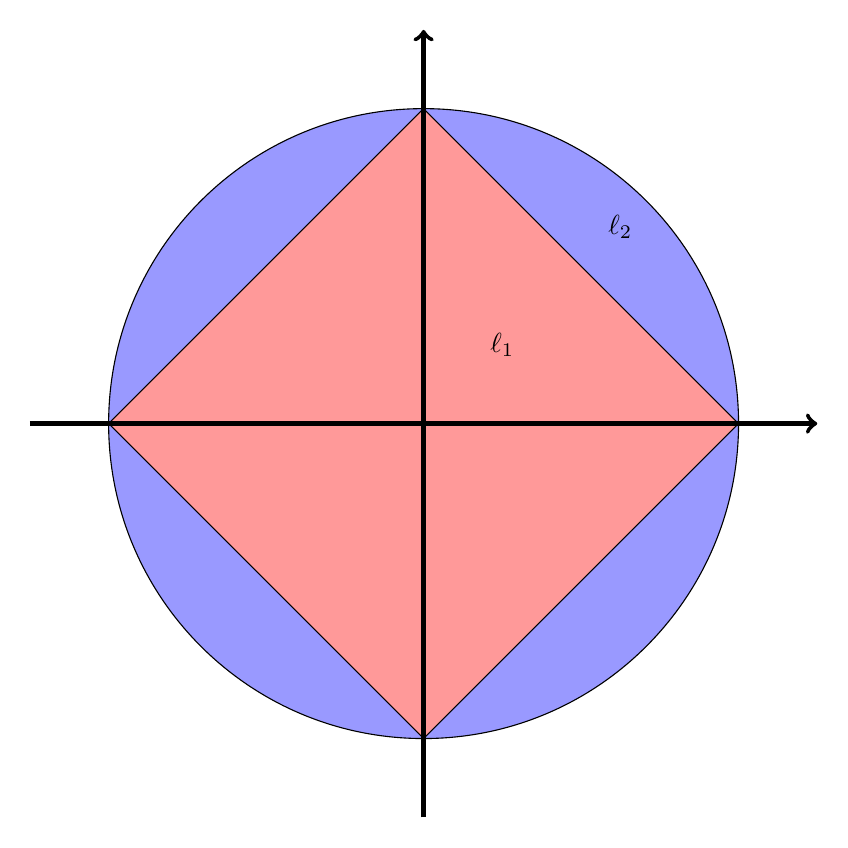
\begin{tikzpicture}

\filldraw[fill=blue!40!white,draw=black] (0,0) circle (4);
\filldraw[fill= red!40!white, draw = black,] (0,4)--(4,0)--(0,-4)--(-4,0)--(0,4);
\draw[->,ultra thick] (-5,0)--(5,0);
\draw[->,ultra thick] (0,-5)--(0,5);
\node[] at (1,1) {$\ell_1$};
\node[] at (2.5,2.5) {$\ell_2$};
\end{tikzpicture}
\end{center}
\item The Lagrange multiplier is defined as $\mathcal{L} (f(x), g(x)) = f(x)-\lambda g(x)$ Where $g(x)$ is our constraint, as such we see that for this problem; 
$$\mathcal{L} (f(x), g(x)) = f(x) + \lambda(\|\xx\|_p-k)$$
We know that minimizing the Lagrangian is equivalent to minimizing the function $f(x)$ subject to the constraint and that $\lambda k$ is not dependent at all upon x, so we can throw this term away; 
$$\text{minimize } \mathcal{L}(f(x), g(x)) = \text{minimize } f(x) + \lambda(\|\xx\|_p)$$
Since we have constructed this from a function and constraint given, we can say that the two statements above are equivalent. 
\item We saw in class that an advantage of the $\ell_1$ norm is it preference for zeros, and we can think of an optimal solution has residing on a vertex of the norm ball. The $\ell_1$ norm will have sparser solutions than the $\ell_2$ norm because it has fewer vertexes, and thus fewer optimal solutions.  
\end{enumerate}
\end{solution}
\newpage



\begin{problem}[Extra Credit]
\textbf{(Lasso)} Show that placing an equal zero-mean Laplace prior on each element of the weights $\thetab$
of a model is equivelent to $\ell_1$ regularization in the Maximum-a-Posteriori estimate
\begin{align*}
    \text{maximize: } & \PP(\thetab | \Dc) = \frac{\PP(\Dc | \thetab)\PP(\thetab)}{\PP(\Dc)}.
\end{align*}
Note the form of the Laplace distribution is
\[
    \mathrm{Lap}(x|\mu,b) = \frac{1}{2b}\exp\left(-\frac{|x-\mu|}{b}\right)
\]
where $\mu$ is the location parameter and $b>0$ controls the variance. Draw (by hand) and compare the density
$\mathrm{Lap}(x|0,1)$ and the standard normal $\Nc(x|0,1)$ and suggest why this would
lead to sparser solutions than a Gaussian prior on each elements of the weights
(which correspond to $\ell_2$ regularization).
\end{problem}
\begin{solution}
\vfill
\end{solution}

\end{document}
